%\begin{itemize}[noitemsep, topsep=0pt]
\documentclass[11pt]{article}

\usepackage{amsmath}
\usepackage{enumitem}
\usepackage{tikz}
\usepackage{cancel}

\usepackage{my_notes}
\usepackage{my_math}

\begin{document}
	General stuff:
	\begin{myitems}
		\item vectors
		\item matrices (det)
        \item test
	\end{myitems}
	
	\section{Basics}
		\subsection{Cartesian Coordinates}
		\subsection{Contour Maps}
		
	\section{2}
		\subsection{Dot Product}
			The dot product of two vectors returns a scalar describing how ....
			The dot product is a derivation from the law of cosines: \\
			%Law of cosines figure
			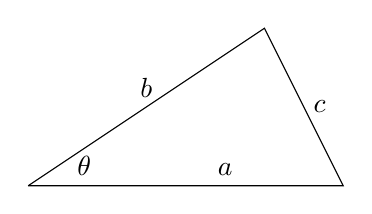
\begin{tikzpicture}
				%\draw [help lines] (0,0) grid (4,2);
				\draw (0,0) -- (3,2) -- (4,0) -- (0,0);
				\node [above right] at (0.5,0) {$\theta$};
				\node [above] at (1.5,1) {$b$};
				\node [right] at (3.5,1) {$c$};
				\node [above] at (2.5,0) {$a$};
			\end{tikzpicture}
			%Law of cosines figure -- vector addition
			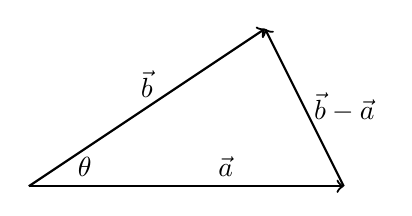
\begin{tikzpicture}
				\draw [thick, ->] (0,0) -- (3,2);
				\draw [thick, ->] (4,0) -- (3,2);
				\draw [thick, ->] (0,0) -- (4,0);
				\node [above right] at (0.5,0) {$\theta$};
				\node [above] at (1.5,1) {$\vec b$};
				\node [right] at (3.5,1) {$\vec b - \vec a$};
				\node [above] at (2.5,0) {$\vec a$};
			\end{tikzpicture}
			%Dot product derivation
			\begin{align*}
				c^2 &= a^2 + b^2 -2ab\cos\theta \\
				\mymag{\vec b - \vec a}^2 &= \mymag{\vec a}^2 + \mymag{\vec b}^2 - 2\mymag{\vec a}\mymag{\vec b}\cos\theta\\
				\vec a = \myvec{a_x,a_y}, \vec b = \myvec{b_x,b_y}\\
				(b_x-a_x)^2 + (b_y-a_y)^2 &= a_x^2 + a_y^2 + b_x^2 + b_y^2 - 2\mymag{\vec a}\mymag{\vec b}\cos\theta\\
				\cancel{b_x^2}-2a_xb_x+\cancel{a_x^2}+\cancel{b_y^2}-2a_yb_y+\cancel{a_y^2}	&= \cancel{a_x^2} + \cancel{a_y^2} + \cancel{b_x^2} + \cancel{b_y^2} - 2\mymag{\vec a}\mymag{\vec b}\cos\theta\\
				a_xb_x+a_yb_y &= \mymag{\vec a}\mymag{\vec b}\cos\theta
			\end{align*}
			We name each side of the resulting equation "the dot product" of the two vectors or $a\cdot b$. Note that $\vec a$ and $\vec b$ could have an arbitrary amount of entries and yield the same result, so:
			\begin{equation}
				a\cdot b = a_0b_0+a_1b_1+...+a_nb_n = \mymag{\vec a}\mymag{\vec b}\cos\theta
			\end{equation}
	\section{Matrices}
		\subsection{What is a Matrix?}
			A Matrix is a rectangle of numbers. For instance,
			$ \begin{bmatrix}
				1 & 2 & 3\\
				2 & 1 & 0
			\end{bmatrix} $
			is a $2 \times 3$ matrix, for it has height $2$ and width $3$.\\
			We can name any given entry $a_{ij}$ where $i$ is its row and $j$ is its column. Generally, 
			$ \begin{bmatrix}
			a_{11} & \dots  & a_{1n}\\
			\vdots & \ddots & \vdots\\
			a_{m1} & \dots  & a_{mn}
			\end{bmatrix} $
			is an $m \times n$ matrix.
		\subsection{Basic Operations}
			\begin{mydes}
				\item{Scaling} The name given to the operation of multiplying every entry within the matrix by a scalar. If a scalar is multiplied to the matrix, the scaling operation is implied.\\ Given a matrix $A$ and scalar $\alpha$, $\alpha \cdot A = 
				\begin{bmatrix}
					\alpha\cdot a_{11} & \dots  & \alpha\cdot a_{1n}\\
					\vdots & \ddots & \vdots\\
					\alpha\cdot a_{m1} & \dots  & \alpha\cdot a_{mn}
				\end{bmatrix}$ \\
				Or, $\alpha \cdot A = \Sigma$
				
				\item{Adding} When two matrices are separated by a ``$+$'' sign, this means that 
			\end{mydes}
		\subsection{Determinant}
		
	\section{Transformations}
\end{document}
